\itemhead{复习题一 · 第7题（教材p.29）}{XJ-B1-C01-RV-P029-Y1165}
\label{XJ-B1-C01-RV-P029-Y1165}
{\footnotesize 湘教版教材p.29 / PDF第36页 / 复习题一 / 第7题}
\field{原题}{已知全集为 $U$，集合 $A,B,C$ 都是 $U$ 的子集，用集合 $U,A,B,C$ 表示图中的阴影部分。
\begin{center}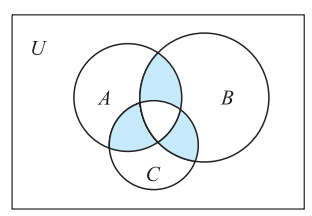
\includegraphics[width=6cm]{figures/C01-RV07.png}\end{center}}
\field{参考答案}{$(A\cap B\cap\complement_U C)\cup(A\cap C\cap\complement_U B)\cup(B\cap C\cap\complement_U A)$，即恰属于三个集合中两个的元素。}
{\small \field{关联知识}{S04 交集、并集及解集的联系（教材帮p.19、20 / PDF28、29）；S05 全集、补集与德摩根律（教材帮p.21 / PDF30）}
\field{方法与易错点}{先各自化简集合或解出约束，再在数轴上合并；有序数对交集通过联立方程求得。 易错：并集重复写元素；连接处一个闭端点也误删；把交集当并集。}
\field{答案依据}{答案册相关题组：PDF第8、9页（册内页7、8）；按当前题库原题逐项重算，不按旧版题号机械对套。}}
